%package list
\documentclass{article}
\usepackage[top=3cm, bottom=3cm, outer=3cm, inner=3cm]{geometry}
\usepackage{multicol}
\usepackage{graphicx}
\usepackage{url}
%\usepackage{cite}
\usepackage{hyperref}
\usepackage{array}
%\usepackage{multicol}
\newcolumntype{x}[1]{>{\centering\arraybackslash\hspace{0pt}}p{#1}}
\usepackage{natbib}
\usepackage{pdfpages}
\usepackage{multirow}
\usepackage[normalem]{ulem}
\useunder{\uline}{\ul}{}
\usepackage{svg}
\usepackage{xcolor}
\usepackage{listings}
\lstdefinestyle{ascii-tree}{
	literate={├}{|}1 {─}{--}1 {└}{+}1 
}
\lstset{basicstyle=\ttfamily,
	showstringspaces=false,
	commentstyle=\color{red},
	keywordstyle=\color{blue}
}
%\usepackage{booktabs}
\usepackage{caption}
\usepackage{subcaption}
\usepackage{float}
\usepackage{array}

\newcolumntype{M}[1]{>{\centering\arraybackslash}m{#1}}
\newcolumntype{N}{@{}m{0pt}@{}}


%%%%%%%%%%%%%%%%%%%%%%%%%%%%%%%%%%%%%%%%%%%%%%%%%%%%%%%%%%%%%%%%%%%%%%%%%%%%
%%%%%%%%%%%%%%%%%%%%%%%%%%%%%%%%%%%%%%%%%%%%%%%%%%%%%%%%%%%%%%%%%%%%%%%%%%%%
\newcommand{\itemStudent}{Reyser Julio Zapata Butron}
\newcommand{\itemCourse}{Programación Web 2}
\newcommand{\itemCourseCode}{20223023}
\newcommand{\itemSemester}{III}
\newcommand{\itemUniversity}{Universidad Nacional de San Agustín de Arequipa}
\newcommand{\itemFaculty}{Facultad de Ingeniería de Producción y Servicios}
\newcommand{\itemDepartment}{Departamento Académico de Ingeniería de Sistemas e Informática}
\newcommand{\itemSchool}{Escuela Profesional de Ingeniería de Sistemas}
\newcommand{\itemAcademic}{2023 - A}
\newcommand{\itemInput}{Del 04 Julio 2023}
\newcommand{\itemOutput}{Al 14 Julio 2023}
\newcommand{\itemPracticeNumber}{07}
\newcommand{\itemTheme}{Relaciones de uno a muchos, muchos a muchos y impresion de pdf y emails}
%%%%%%%%%%%%%%%%%%%%%%%%%%%%%%%%%%%%%%%%%%%%%%%%%%%%%%%%%%%%%%%%%%%%%%%%%%%%
%%%%%%%%%%%%%%%%%%%%%%%%%%%%%%%%%%%%%%%%%%%%%%%%%%%%%%%%%%%%%%%%%%%%%%%%%%%%

\usepackage[english,spanish]{babel}
\usepackage[utf8]{inputenc}
\AtBeginDocument{\selectlanguage{spanish}}
\renewcommand{\figurename}{Figura}
\renewcommand{\refname}{Referencias}
\renewcommand{\tablename}{Tabla} %esto no funciona cuando se usa babel
\AtBeginDocument{%
	\renewcommand\tablename{Tabla}
}

\usepackage{fancyhdr}
\pagestyle{fancy}
\fancyhf{}
\setlength{\headheight}{30pt}
\renewcommand{\headrulewidth}{1pt}
\renewcommand{\footrulewidth}{1pt}
\fancyhead[L]{\raisebox{-0.2\height}{
\includegraphics[width=3cm]{img/logo_episunsa.png}}}
\fancyhead[C]{\fontsize{7}{7}\selectfont	\itemUniversity \\ \itemFaculty \\ \itemDepartment \\ \itemSchool \\ \textbf{\itemCourse}}
\fancyhead[R]{\raisebox{-0.2\height}{
\includegraphics[width=1.2cm]{img/logo_abet}}}
\fancyfoot[L]{Estudiante Reyser Zapata Butron}
\fancyfoot[C]{\itemCourse}
\fancyfoot[R]{Página \thepage}

% para el codigo fuente
\usepackage{listings}
\usepackage{color, colortbl}
\definecolor{dkgreen}{rgb}{0,0.6,0}
\definecolor{gray}{rgb}{0.5,0.5,0.5}
\definecolor{mauve}{rgb}{0.58,0,0.82}
\definecolor{codebackground}{rgb}{0.95, 0.95, 0.92}
\definecolor{tablebackground}{rgb}{0.8, 0, 0}

\lstset{frame=tb,
	language=bash,
	aboveskip=3mm,
	belowskip=3mm,
	showstringspaces=false,
	columns=flexible,
	basicstyle={\small\ttfamily},
	numbers=none,
	numberstyle=\tiny\color{gray},
	keywordstyle=\color{blue},
	commentstyle=\color{dkgreen},
	stringstyle=\color{mauve},
	breaklines=true,
	breakatwhitespace=true,
	tabsize=3,
	backgroundcolor= \color{codebackground},
}

\begin{document}
	
	\vspace*{10px}
	
	\begin{center}	
		\fontsize{17}{17} \textbf{ Informe de Laboratorio
			\itemPracticeNumber}
	\end{center}
	\centerline{\textbf{\Large Tema: \itemTheme}}
	%\vspace*{0.5cm}	
	
	\begin{flushright}
		\begin{tabular}{|M{2.5cm}|N|}
			\hline 
			\rowcolor{tablebackground}
			\color{white} \textbf{Nota}  \\
			\hline 
			\\[30pt]
			\hline 			
		\end{tabular}
	\end{flushright}	
	
	\begin{table}[H]
		\begin{tabular}{|x{4.7cm}|x{4.8cm}|x{4.8cm}|}
			\hline 
			\rowcolor{tablebackground}
			\color{white} \textbf{Estudiantes} & \color{white}\textbf{Escuela}  & \color{white}\textbf{Asignatura}   \\
			\hline 
			{\itemStudent \par \itemEmail} & \itemSchool & {\itemCourse \par Semestre: III} \\
			\hline 			
		\end{tabular}
	\end{table}		
	
	\begin{table}[H]
		\begin{tabular}{|x{4.7cm}|x{4.8cm}|x{4.8cm}|}
			\hline 
			\rowcolor{tablebackground}
			\color{white}\textbf{Laboratorio} & \color{white}\textbf{Tema}  & \color{white}\textbf{Duración}   \\
			\hline 
			\itemPracticeNumber & \itemTheme & 04 horas   \\
			\hline 
		\end{tabular}
	\end{table}
	
	\begin{table}[H]
		\begin{tabular}{|x{4.7cm}|x{4.8cm}|x{4.8cm}|}
			\hline 
			\rowcolor{tablebackground}
			\color{white}\textbf{Semestre académico} & \color{white}\textbf{Fecha de inicio}  & \color{white}\textbf{Fecha de entrega}   \\
			\hline 
			\itemAcademic & \itemInput &  \itemOutput  \\
			\hline 
		\end{tabular}
	\end{table}
	\section{REPOSITORIO DE GITHUB:}
	\begin{itemize}		
		\item Link del Repositorio en github: \url{https://github.com/ReyserLyn/Pweb-lab07.git}
		
		\section{OBJETIVOS:}
		\begin{itemize}		
			\item Desarrollarr los ejercicios en los videos presentados.
			\item Utilizar diferentes librerias para lograr un resultado optimo.
			\item Aprender y produndizar más el Framework Web Django.
			\item Comprender más sobre relaciones en las Bases de Datos.
			
		\end{itemize}
		
		\section{TEMAS:}
		\begin{itemize}		
			\item  Proyectos de Django
			\item Aplicaciones en Django
			\item Base de Datos
			\item Creación de PDF
			\item Envío de Email automatico
		\end{itemize}
		
		
		\section{ACTIVIDADES:}
		Reproducir las actividades de los videos donde trabajamos:
		
		\begin{enumerate}
			\item Relación de uno a muchos
			\item Relación muchos a muchos
			\item Impresión de pdfs
			\item Envio de emails
			\item Crear su video Flipgrid
			
		\end{enumerate}
		
		
	\end{itemize}
	
	\section{EJERCICIOS PROPUESTOS:}
	\begin{enumerate}
		\item Se Deberá replicar las actividades de los video donde se insertar datos y se realizan consultas de una relación de uno a muchos en una base de datos con Django.
		\setcounter{secnumdepth}{0}
		\section{\normalfont\small\href{https://drive.google.com/file/d/1NxYCU2yBtF7KXXwB2iiNtx_zD5NMiTTF/view}{Video de insercion de datos en una BD en relación de uno a muchos (clic)}}\\
		\section{\normalfont\small\href{https://drive.google.com/file/d/1H1uLOHR2qHNH3VcZUd9JpqcACqX0UpoM/view}{Video de querys en una BD en relación de uno a muchos (clic)}} 
		
		Luego de replicar el código del video, ingresamos al shell por defecto de Django con el siguiente comando.
		\lstset{
			backgroundcolor=\color{lightgray!20},
			basicstyle=\ttfamily,
		}
		\begin{lstlisting}
			python .\manage.py shell
		\end{lstlisting}
		\begin{figure}[H]
			\centering
			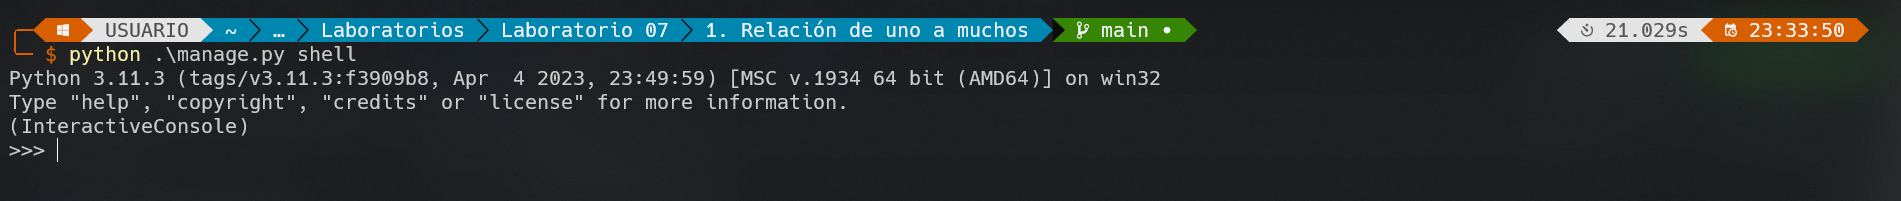
\includegraphics[width=0.8\textwidth,keepaspectratio]{img/Ejercicio1/shell.png}
			%\includesvg{img/automata.svg}
			%\label{img:mot2}
			%\caption{Product backlog.}
		\end{figure}
		
		Ahora que estamos dentro de la shell de nuestro proyecto, podemos empezar insertando datos:
		\begin{lstlisting}
			from example.models import Language, Framework
			javascript = Language(name = 'Javascript')
			javascript.save()
			angular = Framework(name = 'Angular')
			react = Framework(name = 'React')
			javascript
			angular.language = javascript
			react.language = javascript
			angular.save()
			react.save()
			vue = Framework(name='Vue', language=javascript)
			vue.save()
		\end{lstlisting}
		\begin{figure}[H]
			\centering
			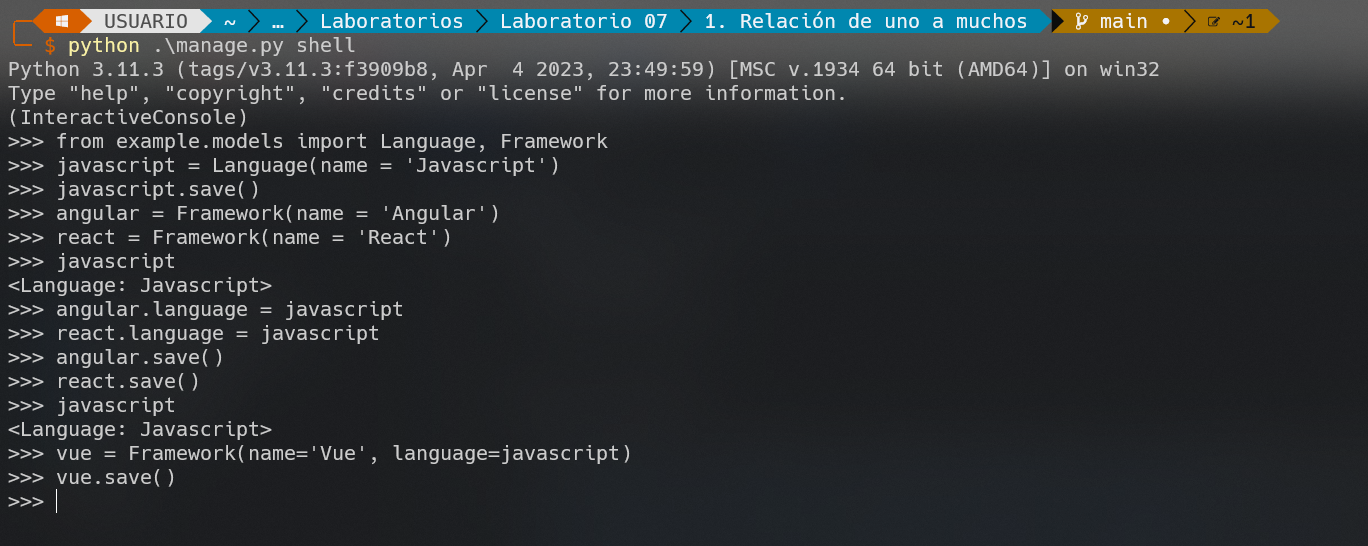
\includegraphics[width=0.8\textwidth,keepaspectratio]{img/Ejercicio1/insert.png}
			%\includesvg{img/automata.svg}
			%\label{img:mot2}
			%\caption{Product backlog.}
		\end{figure}
		Nos fijamos en los cambios que hubo en la base de datos:
		\begin{figure}[H]
			\centering
			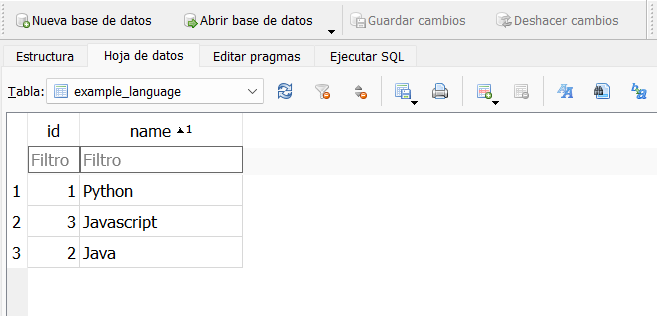
\includegraphics[width=0.8\textwidth,keepaspectratio]{img/Ejercicio1/bd-language.png}
			%\includesvg{img/automata.svg}
			%\label{img:mot2}
			%\caption{Product backlog.}
		\end{figure}
		\begin{figure}[H]
			\centering
			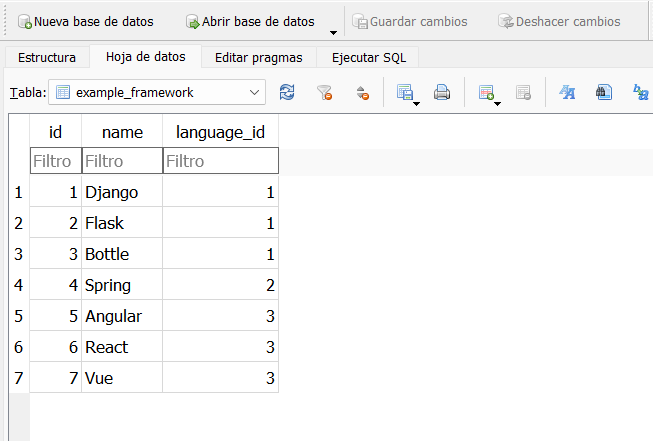
\includegraphics[width=0.8\textwidth,keepaspectratio]{img/Ejercicio1/bd-framework.png}
			%\includesvg{img/automata.svg}
			%\label{img:mot2}
			%\caption{Product backlog.}
		\end{figure}
		Ya que ingresamos datos, podemos hacer las respectivas consultas para la tabla de Framework. Confirmando así que se tiene una relación de Uno a Muchos:
		\begin{lstlisting}
			from example.models import Language, Framework
			Framework.objects.all()
			Framework.objects.filter(language__name='Javascript')
			Framework.objects.filter(language__name='Python')
			Framework.objects.filter(language__name__startswith='Ja')
			Framework.objects.filter(language__name__startswith='C')
		\end{lstlisting}
		\begin{figure}[H]
			\centering
			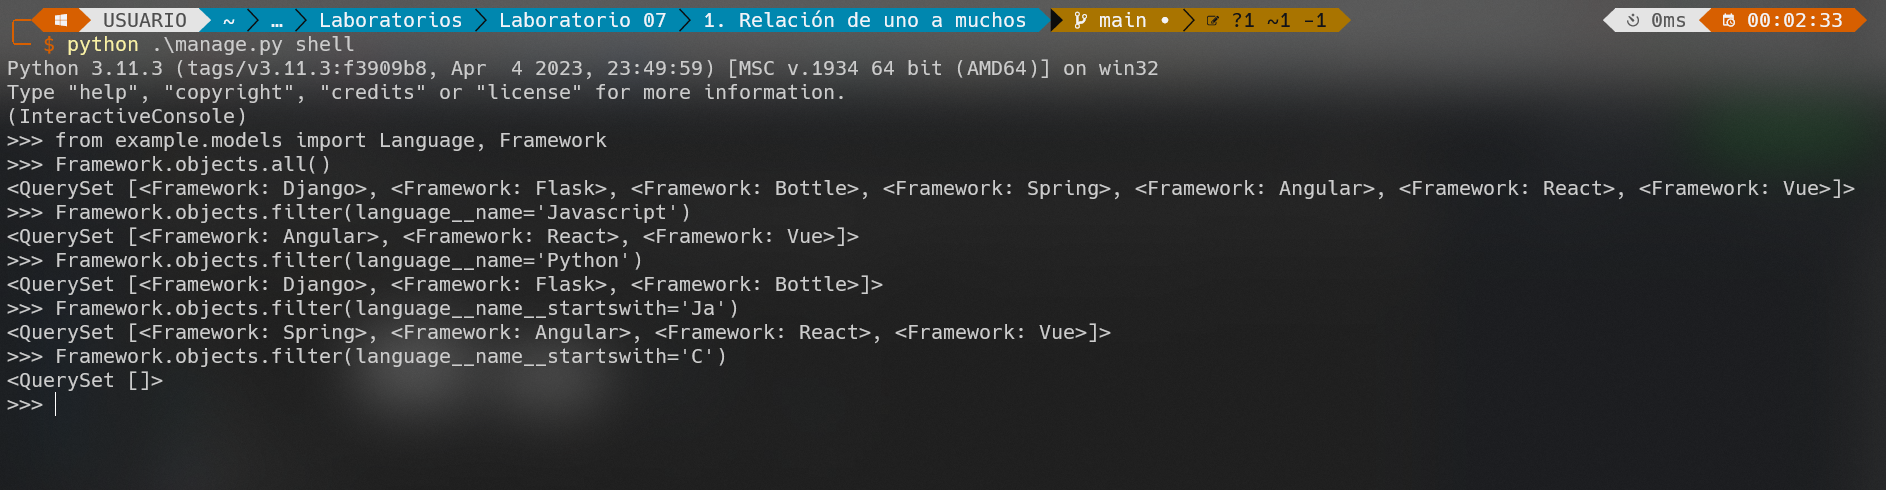
\includegraphics[width=0.8\textwidth,keepaspectratio]{img/Ejercicio1/query-framework.png}
			%\includesvg{img/automata.svg}
			%\label{img:mot2}
			%\caption{Product backlog.}
		\end{figure}
		Ahora realizamos consultas para la tabla de Language:
		\begin{lstlisting}
			from example.models import Language, Framework
			Language.objects.all()
			Language.objects.filter(framework__name='Angular')
			Language.objects.filter(framework__name='Spring')
			Language.objects.filter(framework__name='Django')
		\end{lstlisting}
		\begin{figure}[H]
			\centering
			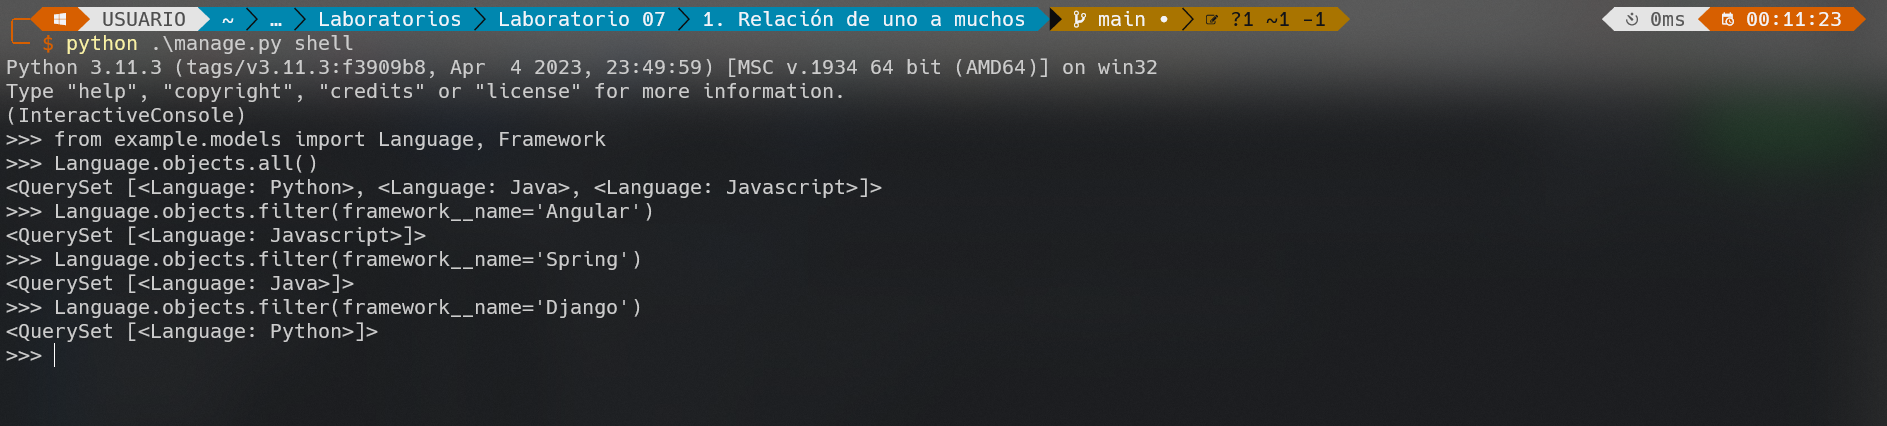
\includegraphics[width=0.8\textwidth,keepaspectratio]{img/Ejercicio1/query-language.png}
			%\includesvg{img/automata.svg}
			%\label{img:mot2}
			%\caption{Product backlog.}
		\end{figure}
		
		\item Se Deberá replicar las actividades de los video donde se insertar datos y se realizan consultas de una relación de muchos a muchos en una base de datos con Django.
		\setcounter{secnumdepth}{0}
		\section{\normalfont\small\href{https://drive.google.com/file/d/1Jpb2xC8gT3R0ZPsn_H1gWBFag8vacoac/view}{Video de insercion de datos en una BD en relación de muchos a muchos (clic)}}\\
		\section{\normalfont\small\href{https://drive.google.com/file/d/16Z8nzSkUnn7K6iTZ4VvAveV37piMwCM2/view}{Video de querys en una BD en relación de muchos a muchos (clic)}} 
		
		Luego de replicar el código del video, ingresamos al shell e insertamos datos:
		\begin{lstlisting}
			from example.models import Movie, Character
			justice_league = Movie(name='Justice League')
			justice_league.save()
			superman = Character(name='Superman')
			superman.save()
			superman.movies.add(justice_league)
			flash = Movie(name='Flash')
			wonder_woman = Movie(name='Wonder Woman 1984')
			flash_character = Character(name = 'Flash')
			flash.save()
			wonder_woman.save()
			flash_character.save()
			flash_character.movies.add(flash)
			superman.movies.add(wonder_woman)
			flash_character.movies.add(justice_league)
			superman.movies.create(name='El hombre de acero')
		\end{lstlisting}
		\begin{figure}[H]
			\centering
			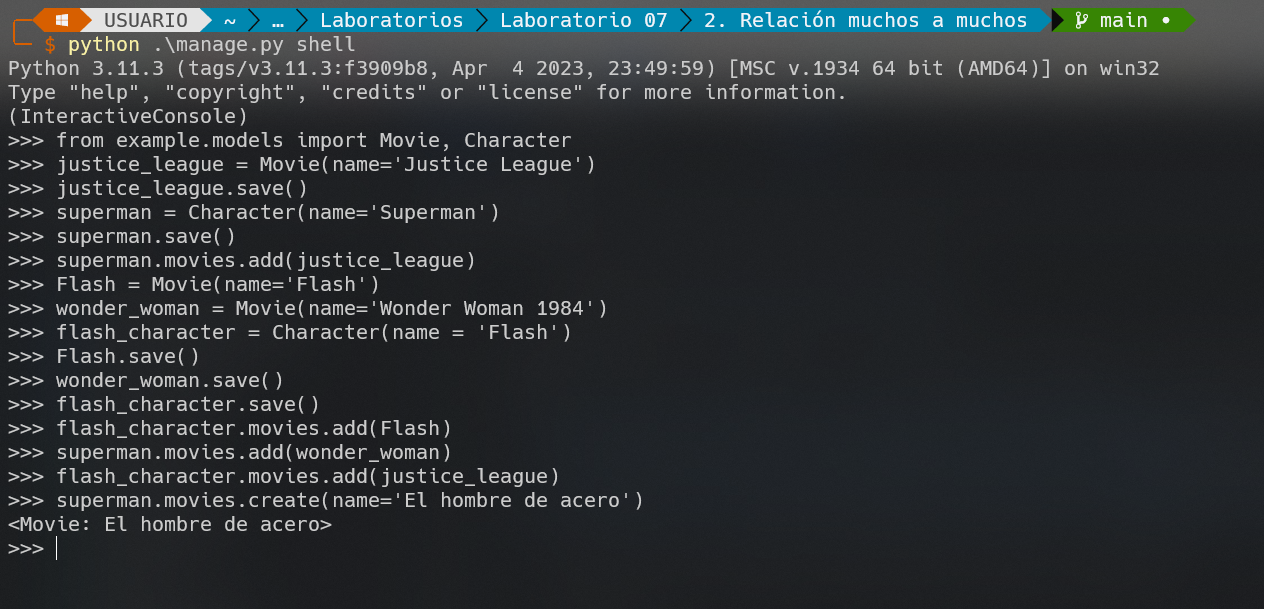
\includegraphics[width=0.8\textwidth,keepaspectratio]{img/Ejercicio2/insert.png}
			%\includesvg{img/automata.svg}
			%\label{img:mot2}
			%\caption{Product backlog.}
		\end{figure}
		Ahora revisamos los cambios que hubo en la base de datos:
		\begin{figure}[H]
			\centering
			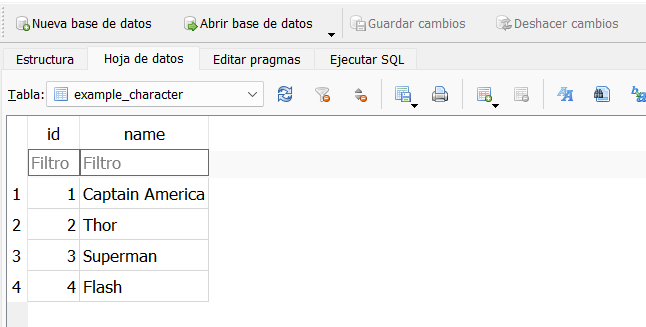
\includegraphics[width=0.8\textwidth,keepaspectratio]{img/Ejercicio2/bd-character.png}
			%\includesvg{img/automata.svg}
			%\label{img:mot2}
			%\caption{Product backlog.}
		\end{figure}
		\begin{figure}[H]
			\centering
			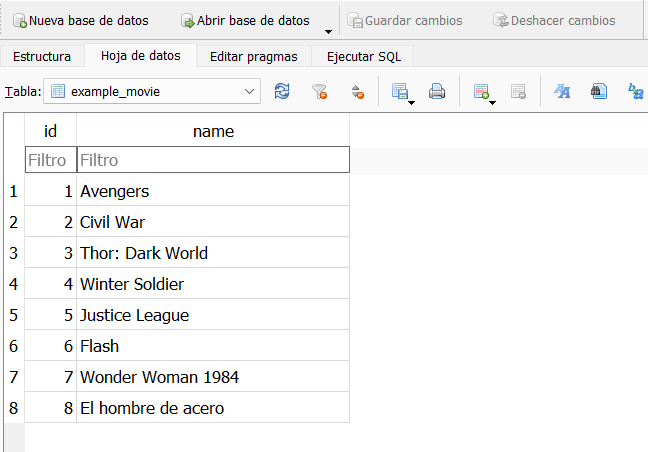
\includegraphics[width=0.8\textwidth,keepaspectratio]{img/Ejercicio2/bd-movie.png}
			%\includesvg{img/automata.svg}
			%\label{img:mot2}
			%\caption{Product backlog.}
		\end{figure}
		\begin{figure}[H]
			\centering
			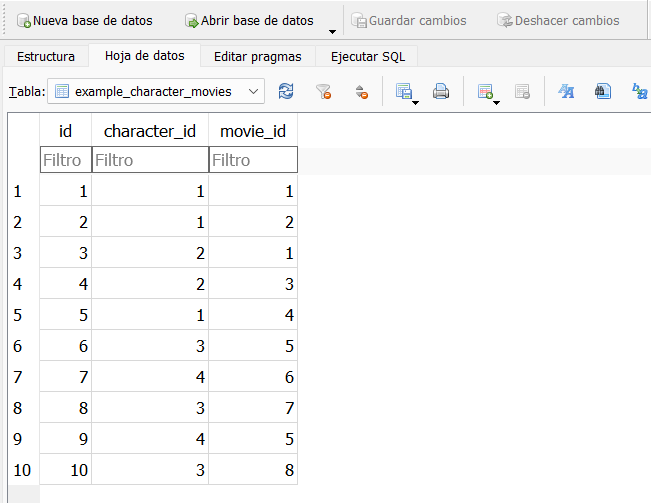
\includegraphics[width=0.8\textwidth,keepaspectratio]{img/Ejercicio2/bd-character-movie.png}
			%\includesvg{img/automata.svg}
			%\label{img:mot2}
			%\caption{Product backlog.}
		\end{figure}
		Por ultimo, realizamos los querys para estas tablas y confirmamos su relación de muchos a muchhos, siendo gran ejemplo, Superman y Justice League
		\begin{lstlisting}
			from example.models import Movie, Character
			Character.objects.all()
			Character.objects.filter(movies__name='Justice League')
			Movie.objects.filter(character__name='Superman')
			superman = Character.objects.get(name='Superman')
			superman.movies.all()
			justice_league = Movie.objects.get(name='Justice League')
			justice_league.character_set.all()
			flash = Character.objects.get(name='Flash')
			flash.movies.all()
		\end{lstlisting}
		\begin{figure}[H]
			\centering
			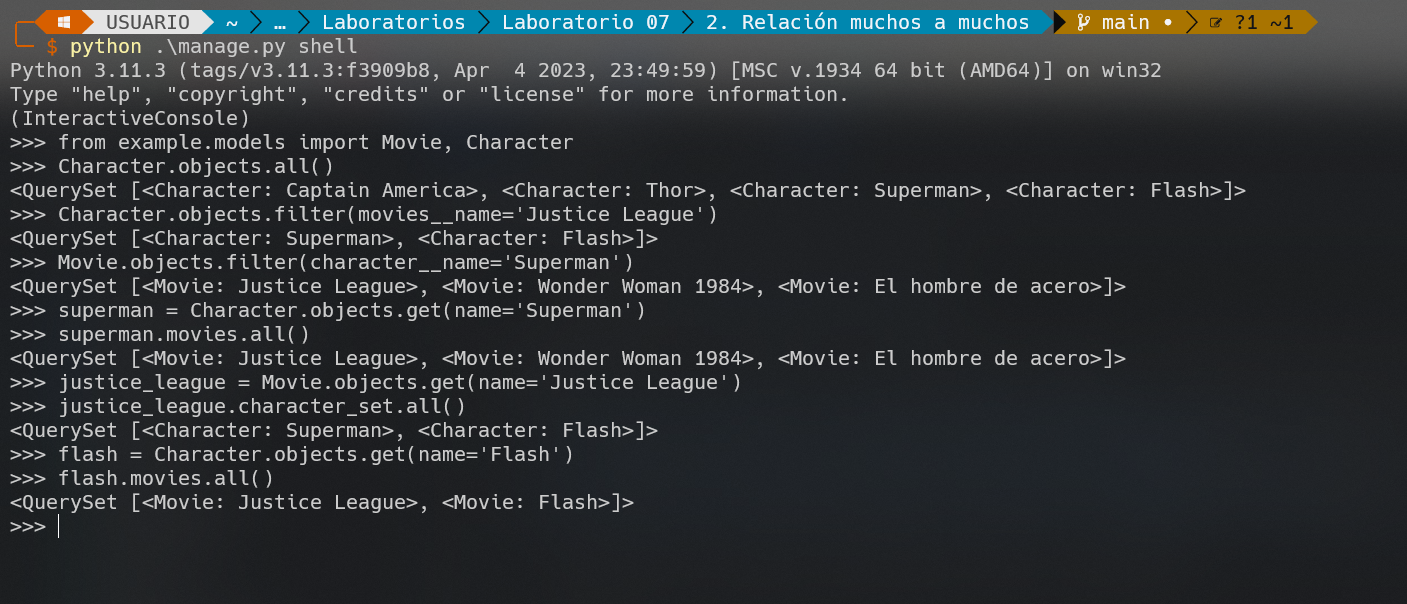
\includegraphics[width=0.8\textwidth,keepaspectratio]{img/Ejercicio2/query.png}
			%\includesvg{img/automata.svg}
			%\label{img:mot2}
			%\caption{Product backlog.}
		\end{figure}
		\item Se deberá replicar el código del siguiente video con la intención de aprender sobre la creación e impresión de pdfs con Django
		\setcounter{secnumdepth}{0}
		\section{\normalfont\small\href{https://drive.google.com/file/d/1btSc7p5O_ll0CBdiLokWi89lq5yXahoN/view}{Render a Django HTML Template to a PDF file Django Utility CFE Render_to_PDF(clic)}}
		
		Se logró replicar el código siendo estos los más importantes
		\begin{description}
			[--] utils.py, es el encargado de renderizar el pdf, transformando el Html en un PDF.
			\begin{figure}[H]
				\centering
				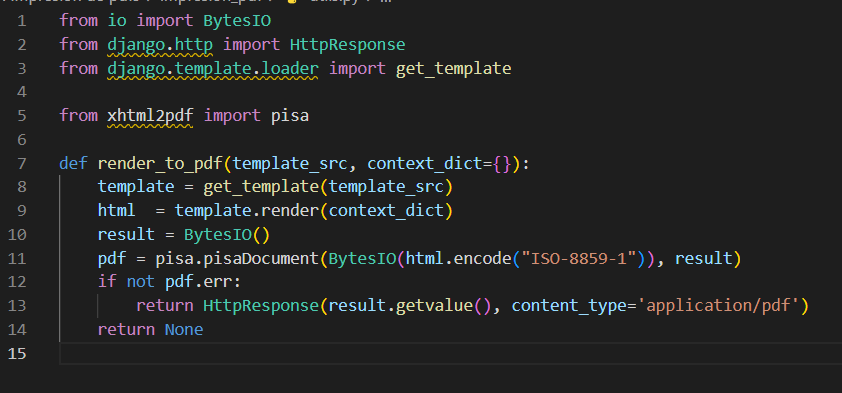
\includegraphics[width=0.8\textwidth,keepaspectratio]{img/Ejercicio3/utils.png}
				%\includesvg{img/automata.svg}
				%\label{img:mot2}
				%\caption{Product backlog.}
			\end{figure}
			
			[--] views.py, este es el encargado de generar el pdf, dando el nombre y la información necesario al template para que esté completo.
			\begin{figure}[H]
				\centering
				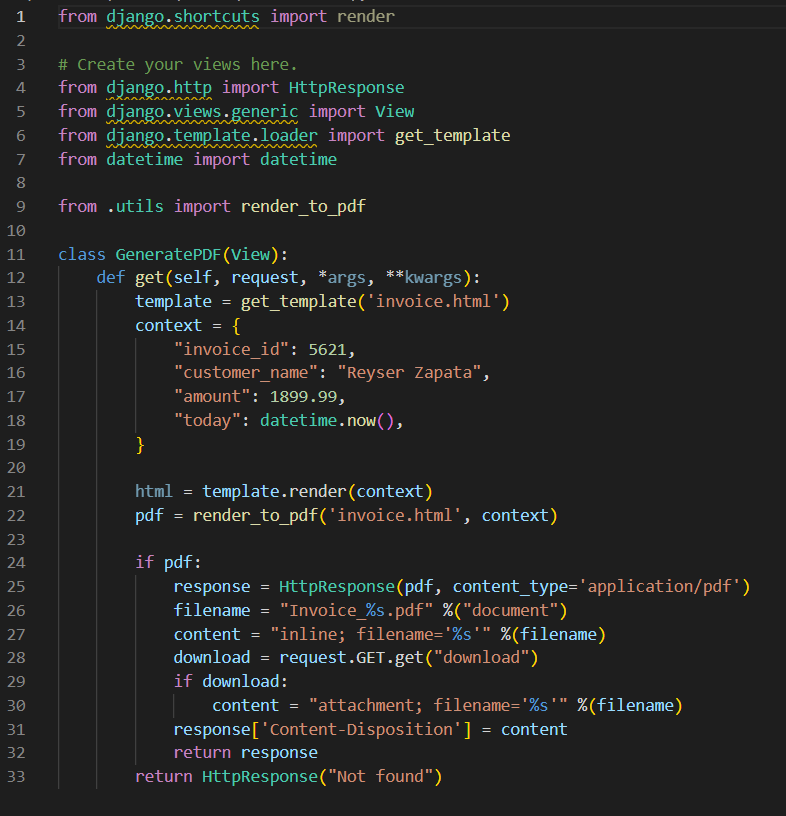
\includegraphics[width=0.8\textwidth,keepaspectratio]{img/Ejercicio3/view.png}
				%\includesvg{img/automata.svg}
				%\label{img:mot2}
				%\caption{Product backlog.}
			\end{figure}
			[--] template.html, es lo que recibirá información de la Vista y se transformará en PDF
			\begin{figure}[H]
				\centering
				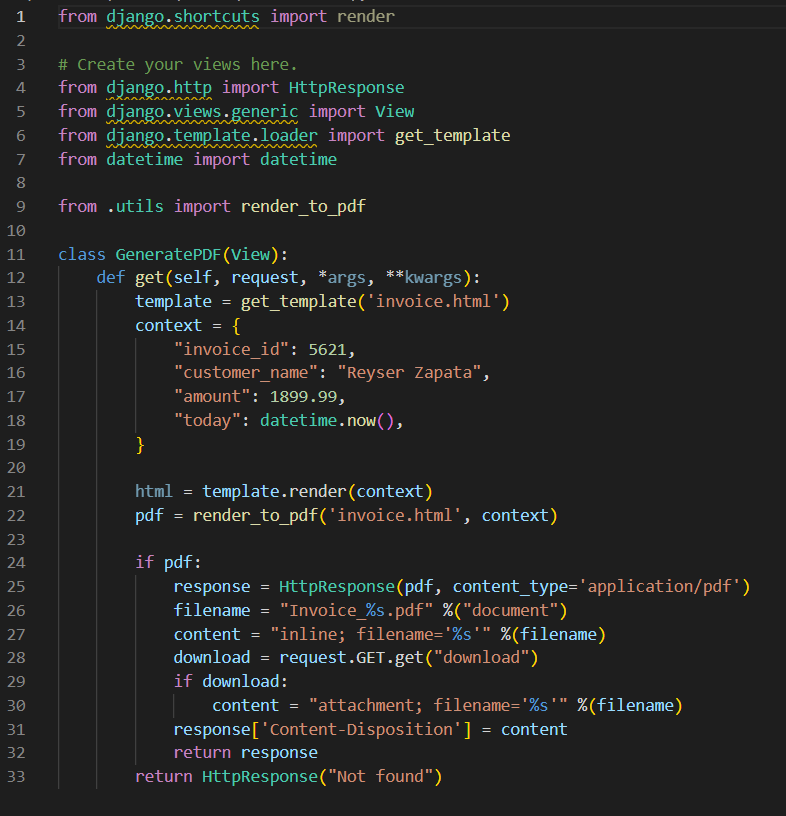
\includegraphics[width=0.8\textwidth,keepaspectratio]{img/Ejercicio3/view.png}
				%\includesvg{img/automata.svg}
				%\label{img:mot2}
				%\caption{Product backlog.}
			\end{figure}
			Para poder ejecutar este ejercicio, necesitaremos seguir los siguientes pasos para poder ejecutarlo:
			\begin{lstlisting}
				py -m venv venv
			\end{lstlisting}
			\begin{lstlisting}
				pip install -r requirements.txt
			\end{lstlisting}
			\begin{lstlisting}
				python .\manage.py runserver
			\end{lstlisting}
			Una vez hayamos seguido los comandos, podremos abrir el servidor local (\url{http://127.0.0.1:8000/})y ver nuestro PDF
			\begin{figure}[H]
				\centering
				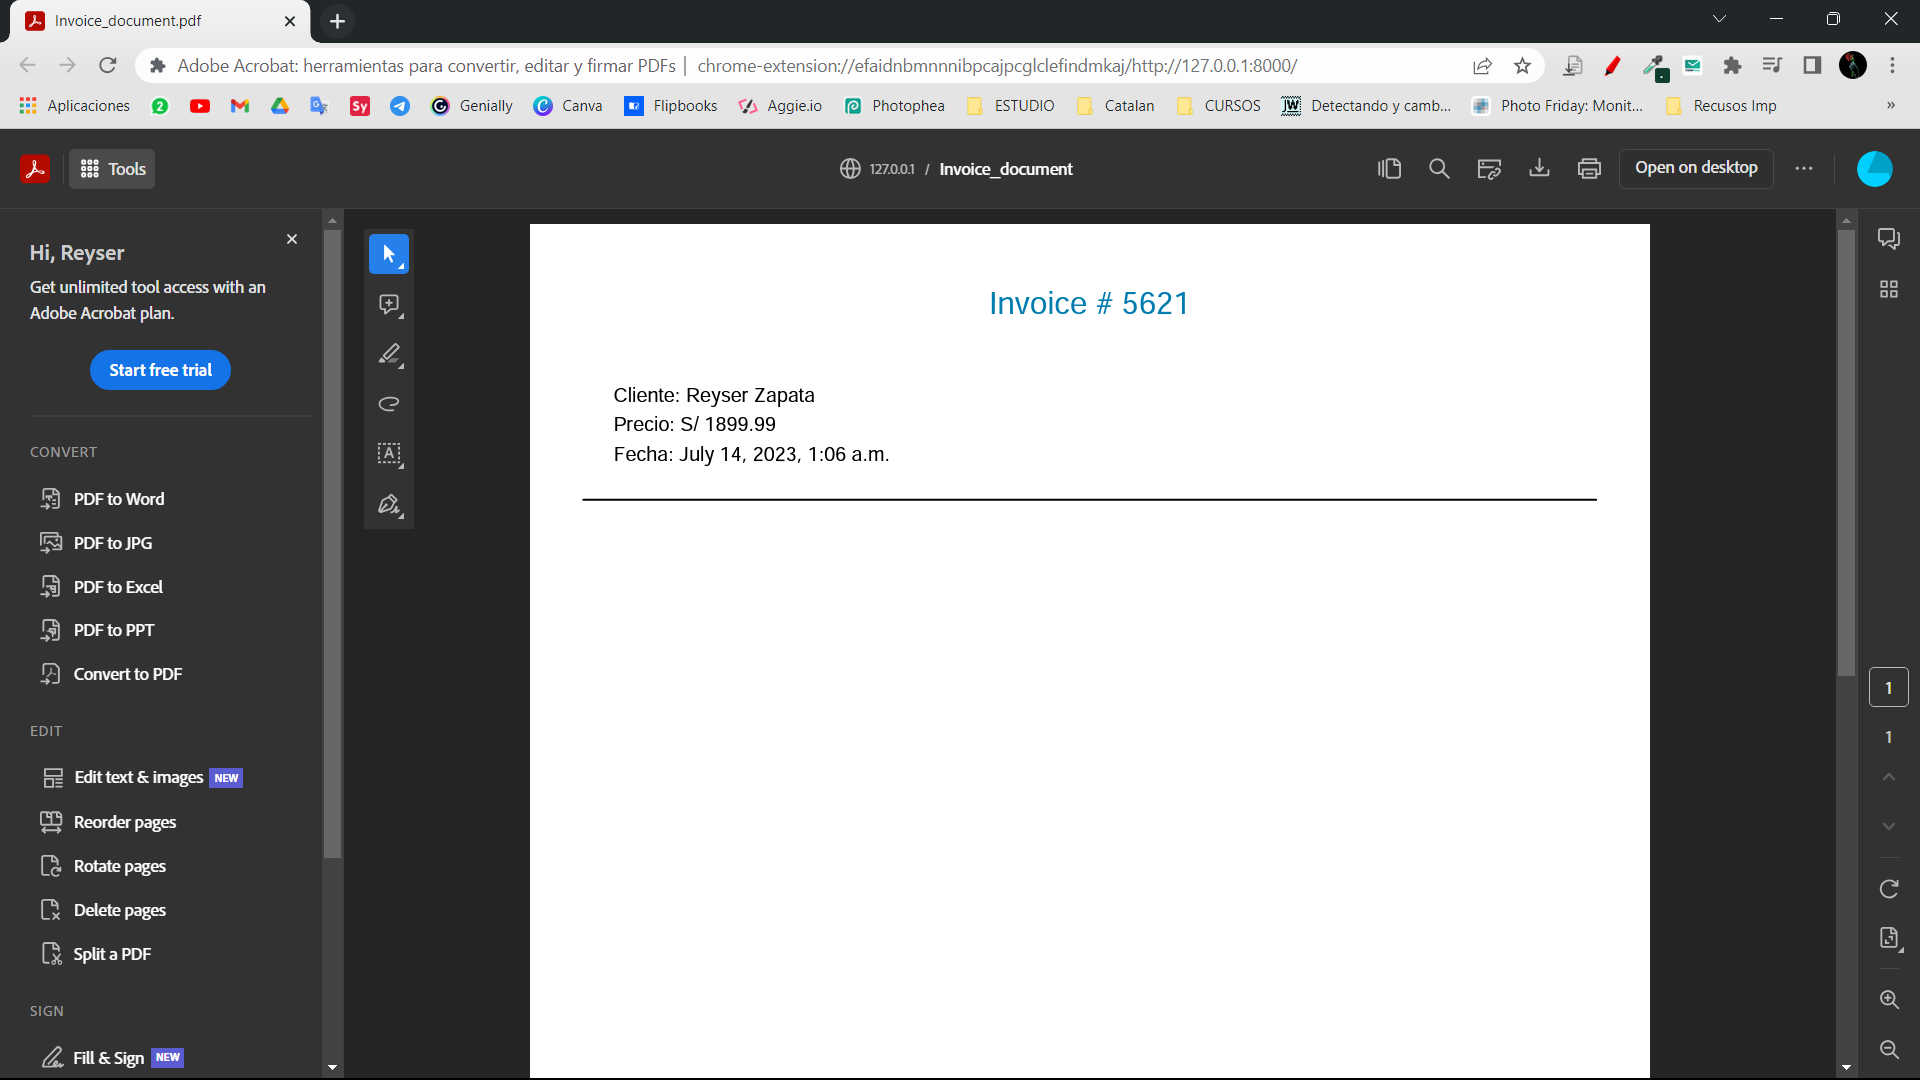
\includegraphics[width=0.8\textwidth,keepaspectratio]{img/Ejercicio3/pdf.png}
				%\includesvg{img/automata.svg}
				%\label{img:mot2}
				%\caption{Product backlog.}
			\end{figure}
		\end{description}
		
		\item--Se deberá replicar el código del siguiente video con la intención de aprender sobre el envio de Email automaticamente con Django
		
		\setcounter{secnumdepth}{0}
		\section{\normalfont\small\href{https://drive.google.com/file/d/1JueuRhWgnXUNERTWK77lqQQgeqF1xkhK/view}{Sendings Emails in Django (clic)}}\\
		
		Se logró replicar el código, un proyecto y una app en Djgango, siendo los archivos más importantes los siguientes:
		
		\begin{description}
			[--] views.py, aqui debemos colocar el Asunto, el Cuerpo, el Correo con el que se enviará y el/los correo(s) a donde llegará(destinatario). Para el ejemplo se usará correos temporales como destinatarios.
			\begin{figure}[H]
				\centering
				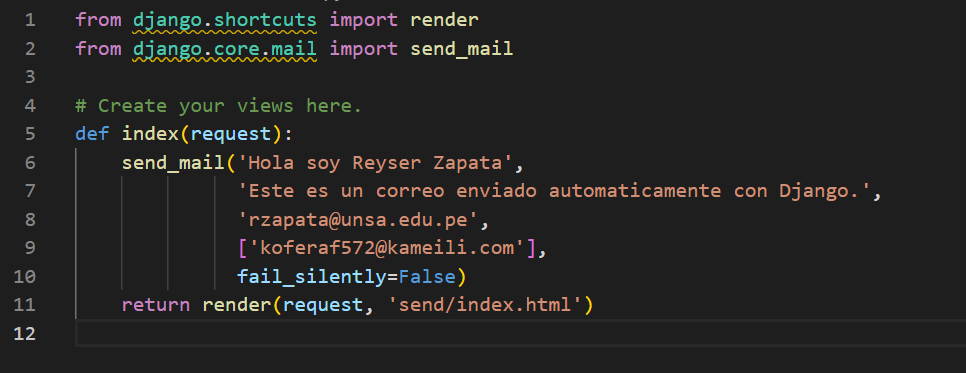
\includegraphics[width=0.8\textwidth,keepaspectratio]{img/Ejercicio4/view.png}
				%\includesvg{img/automata.svg}
				%\label{img:mot2}
				%\caption{Product backlog.}
			\end{figure}
			[--] settings.py, aqui debemos configurar el servicio SMTP del cual haremos uso para el envío de correo, en el que debemos de colocar, dominio, puerto y el correo(user) junto con la contraseña con la que se enviará el correo, es importante que estos sean correctos. Algo importante para que funcione con el servicio SMTP de Gmail, es habilitar el acceso de aplicaciones menos seguras en tu cuenta de Gmail. Puedes hacerlo siguiendo estas instrucciones: \url{https://support.google.com/accounts/answer/6010255}
			
			\begin{figure}[H]
				\centering
				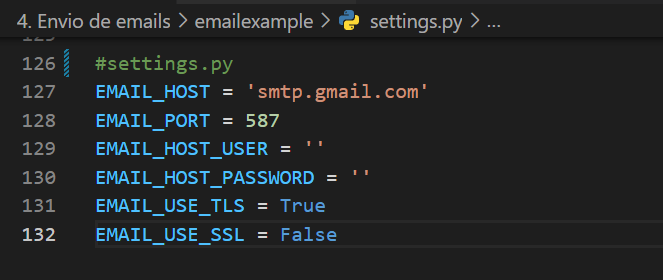
\includegraphics[width=0.8\textwidth,keepaspectratio]{img/Ejercicio4/settings.png}
				%\includesvg{img/automata.svg}
				%\label{img:mot2}
				%\caption{Product backlog.}
			\end{figure}
			[--] index.html, si todo va bien, esta página se cargará correctamente:
			\begin{figure}[H]
				\centering
				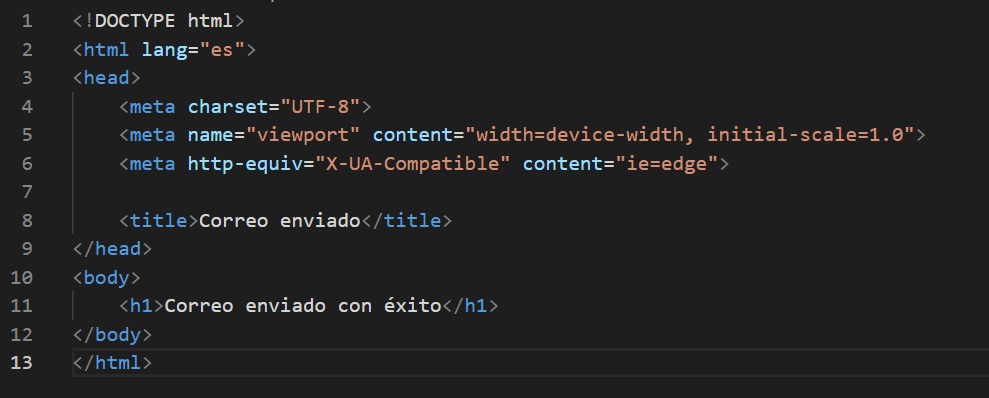
\includegraphics[width=0.8\textwidth,keepaspectratio]{img/Ejercicio4/index.png}
				%\includesvg{img/automata.svg}
				%\label{img:mot2}
				%\caption{Product backlog.}
			\end{figure}
		\end{description}
		Para poder ejecutar este ejercicio, necesitaremos seguir los siguientes pasos para poder ejecutarlo:
		\begin{lstlisting}
			python .\manage.py runserver
		\end{lstlisting}
		Una vez hayamos seguido los comandos, podremos abrir el servidor local (\url{http://127.0.0.1:8000/}) y comprobar si se ha enviado el email
		\begin{figure}[H]
			\centering
			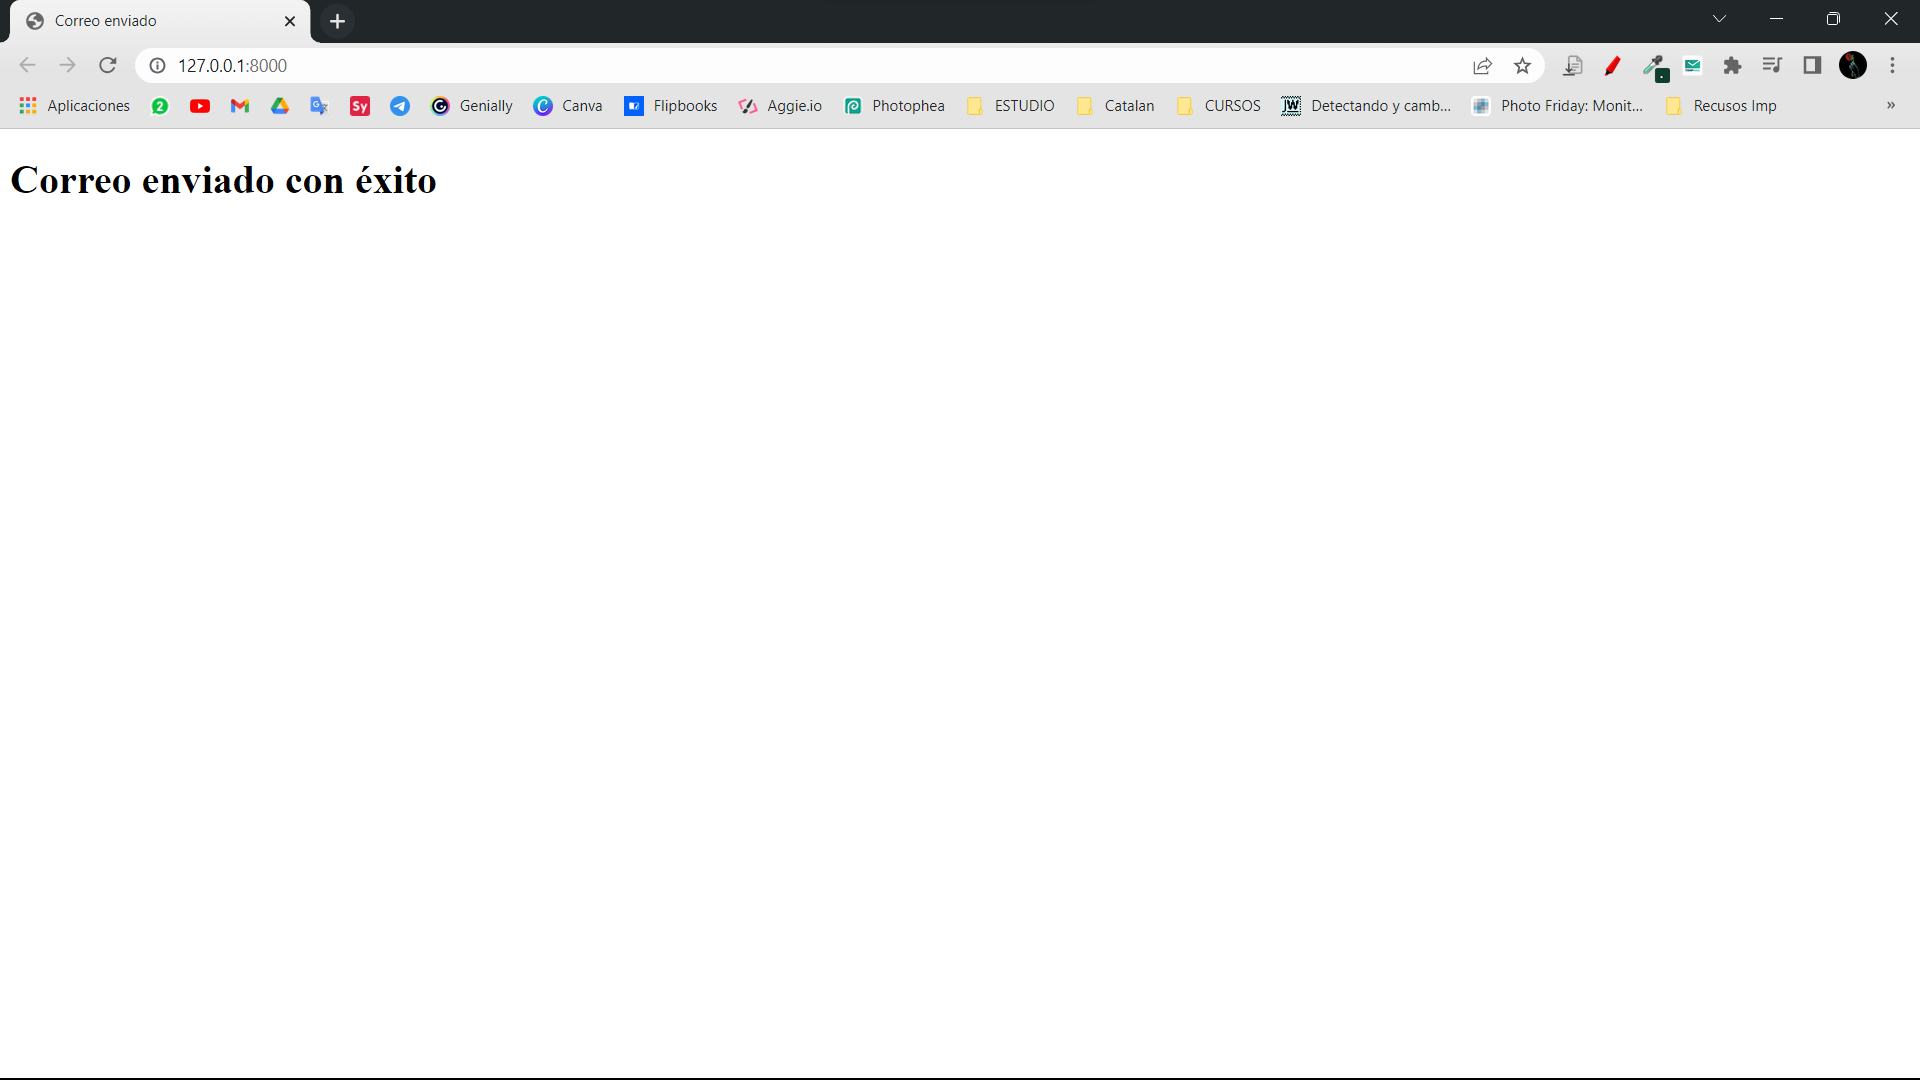
\includegraphics[width=0.8\textwidth,keepaspectratio]{img/Ejercicio4/email-page.png}
			%\includesvg{img/automata.svg}
			%\label{img:mot2}
			%\caption{Product backlog.}
		\end{figure}
		\begin{figure}[H]
			\centering
			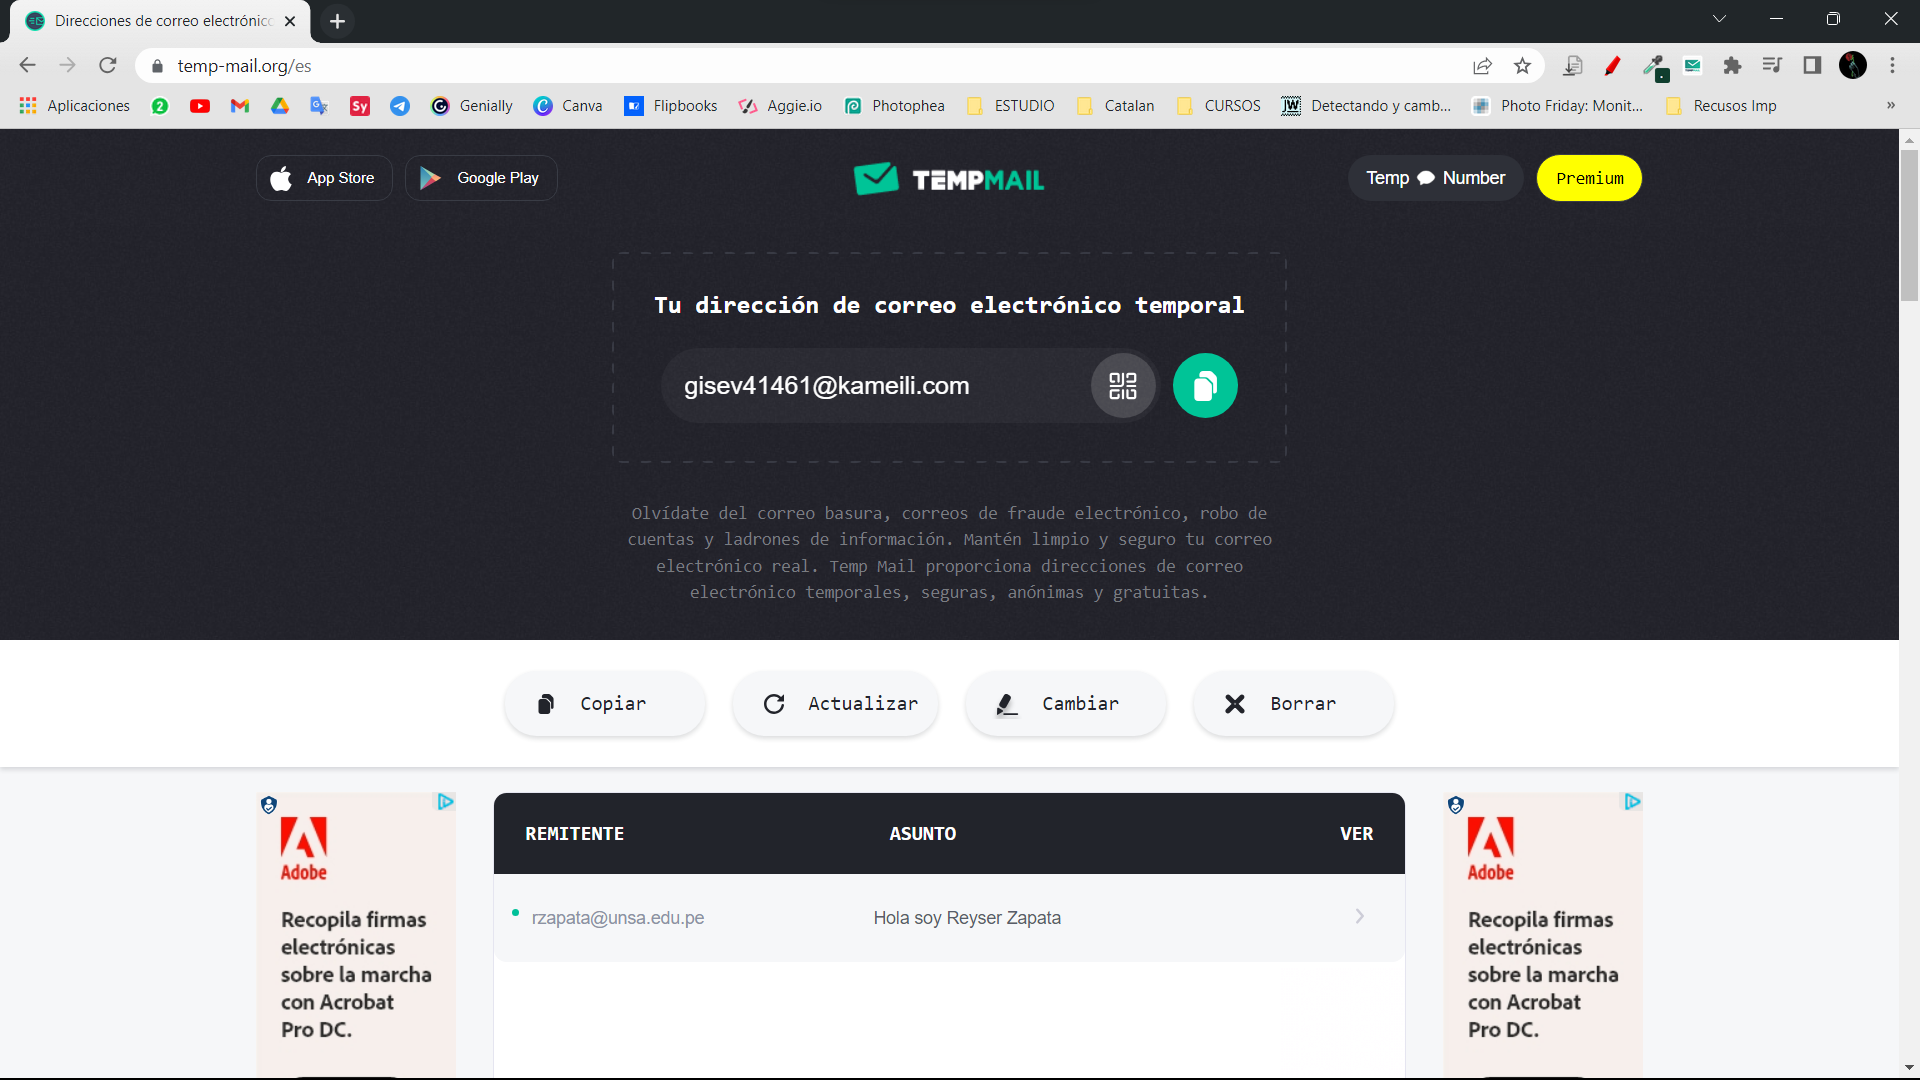
\includegraphics[width=0.8\textwidth,keepaspectratio]{img/Ejercicio4/email-received1.png}
			%\includesvg{img/automata.svg}
			%\label{img:mot2}
			%\caption{Product backlog.}
		\end{figure}
		\begin{figure}[H]
			\centering
			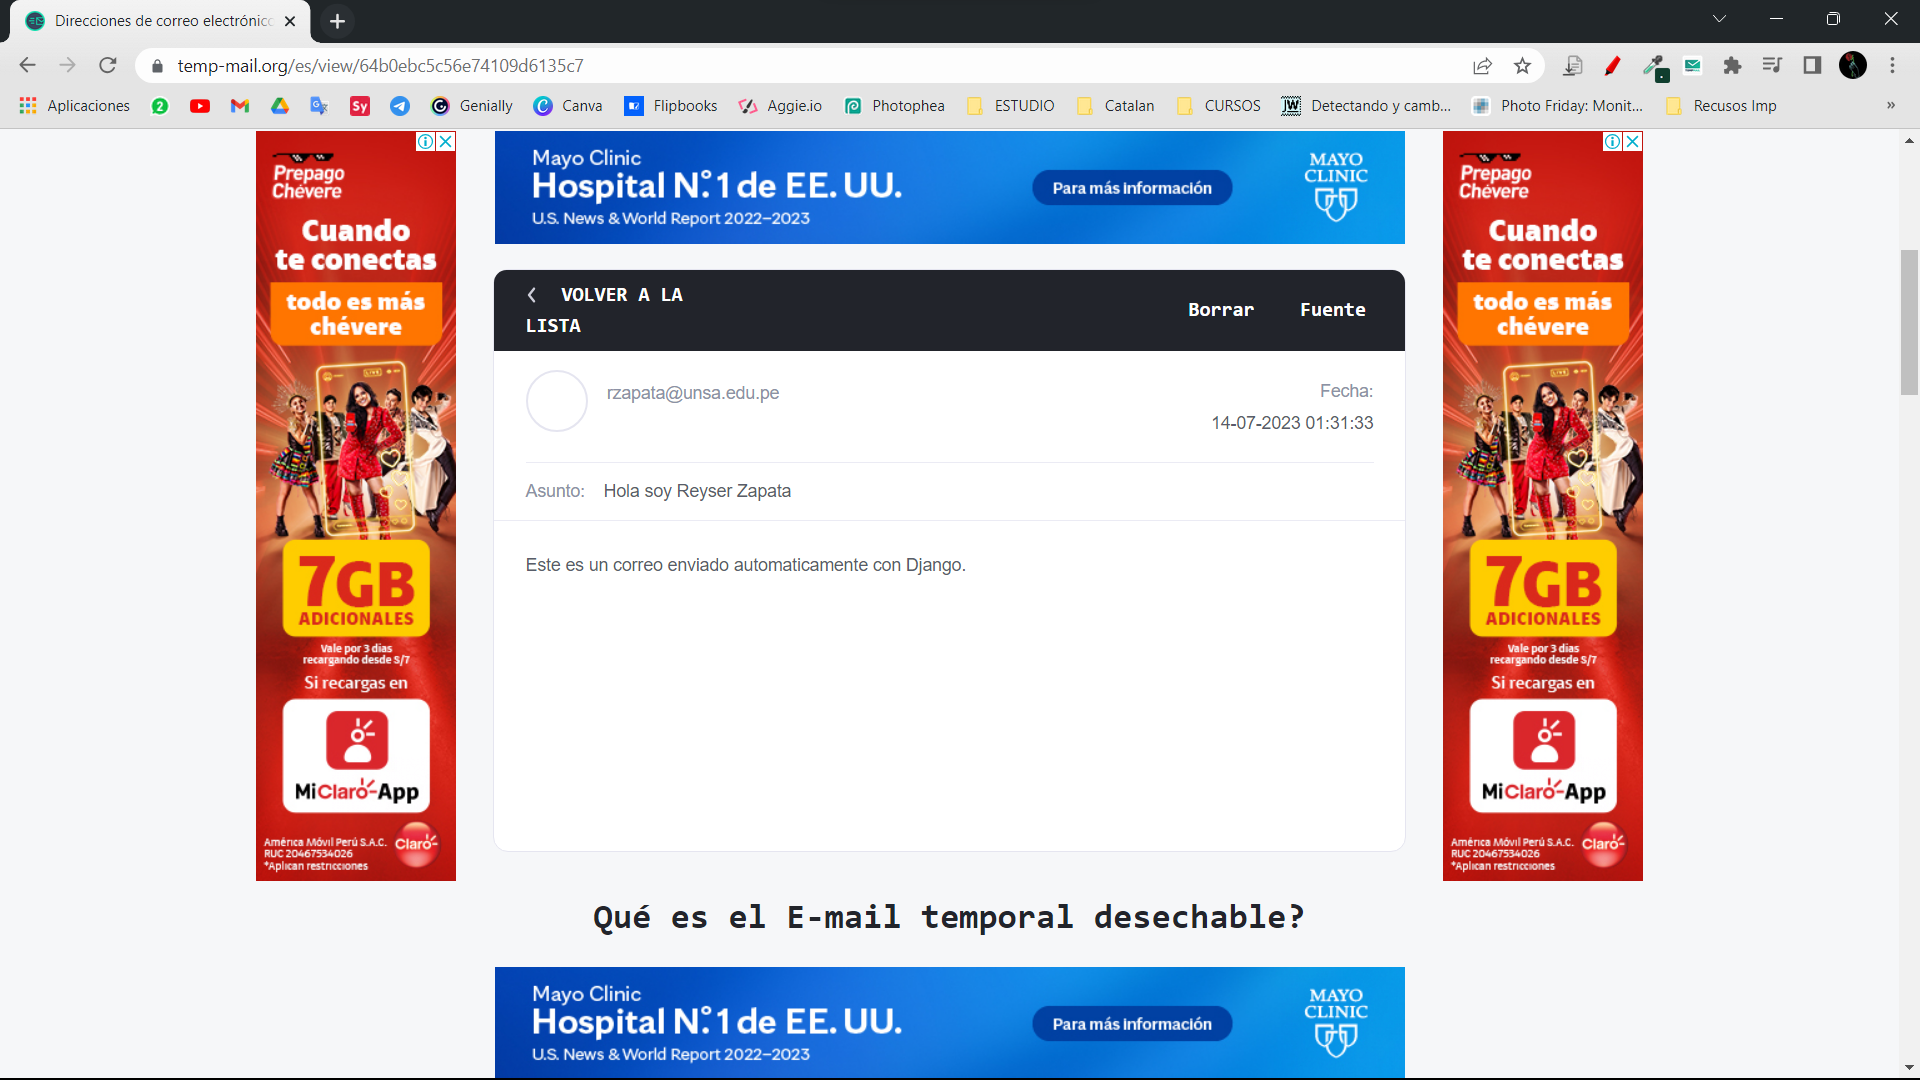
\includegraphics[width=0.8\textwidth,keepaspectratio]{img/Ejercicio4/email-received2.png}
			%\includesvg{img/automata.svg}
			%\label{img:mot2}
			%\caption{Product backlog.}
		\end{figure}
		\item Realizar un video Flipgrid mostrando las ejecuciones de los ejercicios:
		\begin{description}
			[--] \setcounter{secnumdepth}{0}
			\section{\normalfont\small\href{https://flip.com/s/VpYRDah9wroh}{Link del video (clic): https://flip.com/s/VpYRDah9wroh}}\\
		\end{description}
		
		\section{COMMITS IMPORTANTES EN GITHUB:}
		Para este Laboratorio, se necesitó de varios commits, en los cuales se puede apreciar el progreso que hubo para poder completar con éxito este laboratorio. En cada commit se logró implementar un ejercicio de este laboratorio.
		\begin{figure}[H]
			\centering
			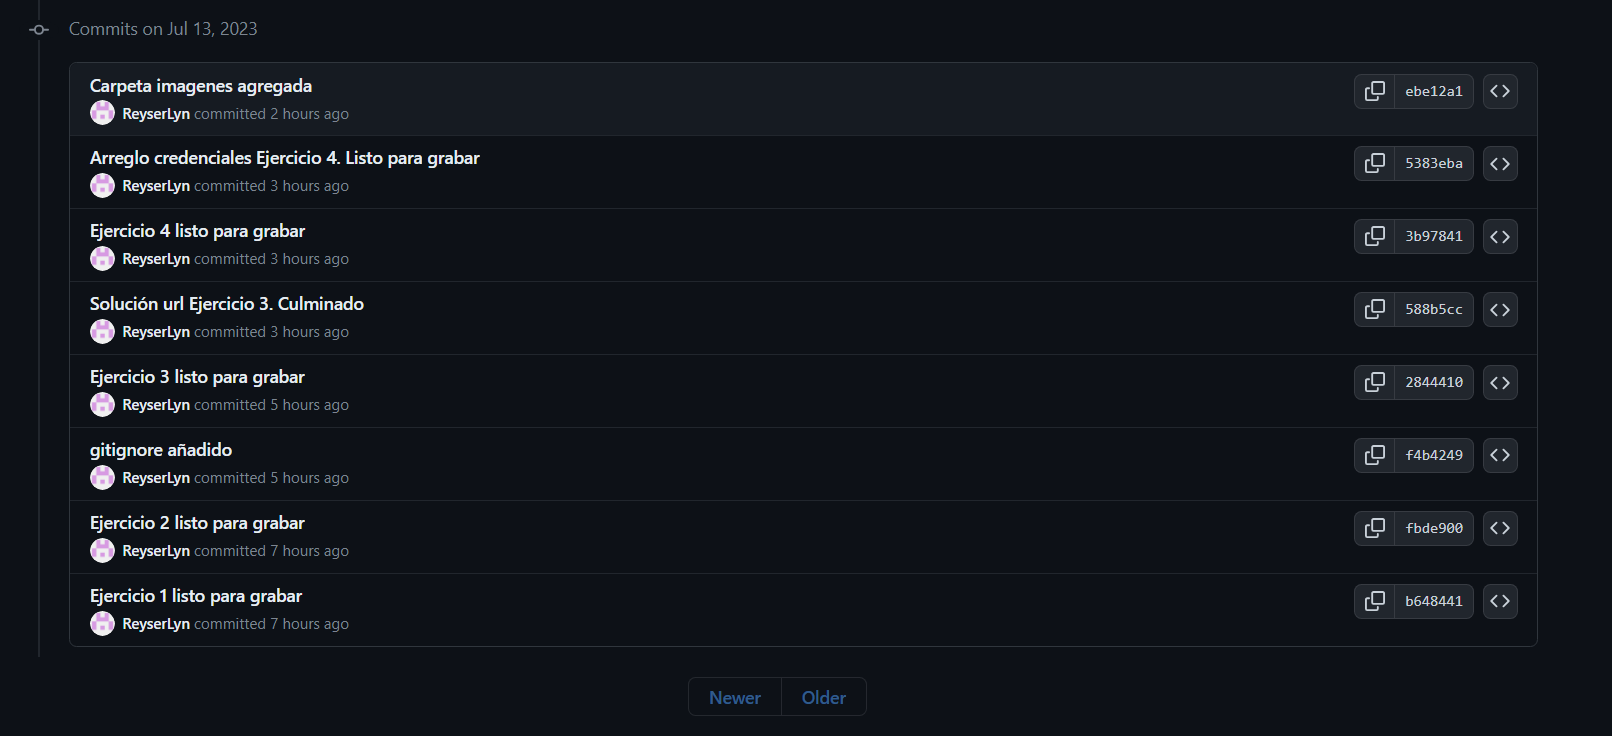
\includegraphics[width=0.8\textwidth,keepaspectratio]{img/Commits.png}
			%\includesvg{img/automata.svg}
			%\label{img:mot2}
			%\caption{Product backlog.}
		\end{figure}
		\section{AUTOEVALUACIÓN INDIVIDUAL:}
		\begin{figure}[H]
			\centering
			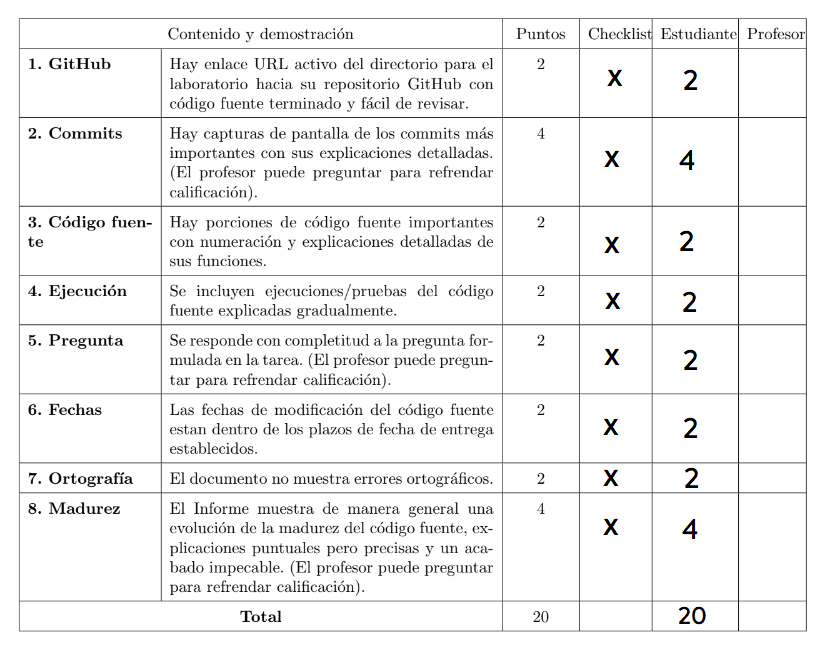
\includegraphics[width=0.8\textwidth,keepaspectratio]{img/Autocalificacion.png}
			%\includesvg{img/automata.svg}
			%\label{img:mot2}
			%\caption{Product backlog.}
		\end{figure}
	\end{enumerate}
	\section{Referencias}
	\begin{itemize}			
		
		\item \url{https://www.w3schools.com/python/python_reference.asp}
		\item \url{https://docs.python.org/3/tutorial/}
		\item \url{https://docs.djangoproject.com/es/4.2/}
	\end{itemize}
	%\clearpage
	%\bibliographystyle{apalike}
	%\bibliographystyle{IEEEtranN}
	%\bibliography{bibliography}
	
\end{document} 